

\subsection{クライアントサイドの実装}\label{4.1.2}
クライアントサイドでは,WebAPIを利用してWebアプリケーションを実装した.
Webアプリケーションのフレームワークとして,Next.jsを採用した.
Next.jsはReact.jsをベースにしており,React.jsの開発を効率化に加え,サーバーサイドによるレンダリングのサポートによってSEO対策やパフォーマンスの向上を実現できる.
React.jsはJavaScriptのライブラリであり,コンポーネントベースのアーキテクチャを採用している.
コンポーネントを独立した単位として開発すると,開発者はそれぞれのコンポーネントに集中できるため開発効率が向上する.
コンポーネントは再利用可能な単位であり複数のページで同じコンポーネントが利用でき,これにより開発コストを削減し保守性を向上させる.
またReactは仮想DOMを採用しており実際のDOM(Document Object Model)を操作する代わりに、JavaScriptのオブジェクトとして扱う仕組みである.
仮想DOMは実際のDOMと比較して,更新が必要な部分だけを計算を行うためパフォーマンスの向上が図れる.



基本的に既存の滞在ウォッチで同じように滞在者,滞在履歴,利用者情報のページが存在する.
変更点として在室時間をガントチャートで可視化している画面が挙げられる.
図\ref{fig:gantt}にその画面を示す.
この画面の緑の部分にカーソルを合わせると,入室時間と退室時間を確認できる.
日付と部屋を指定するタブがあり,そのタブに応じたそれぞれのデータを表示される.

\begin{figure}[tbh]
  \centering
  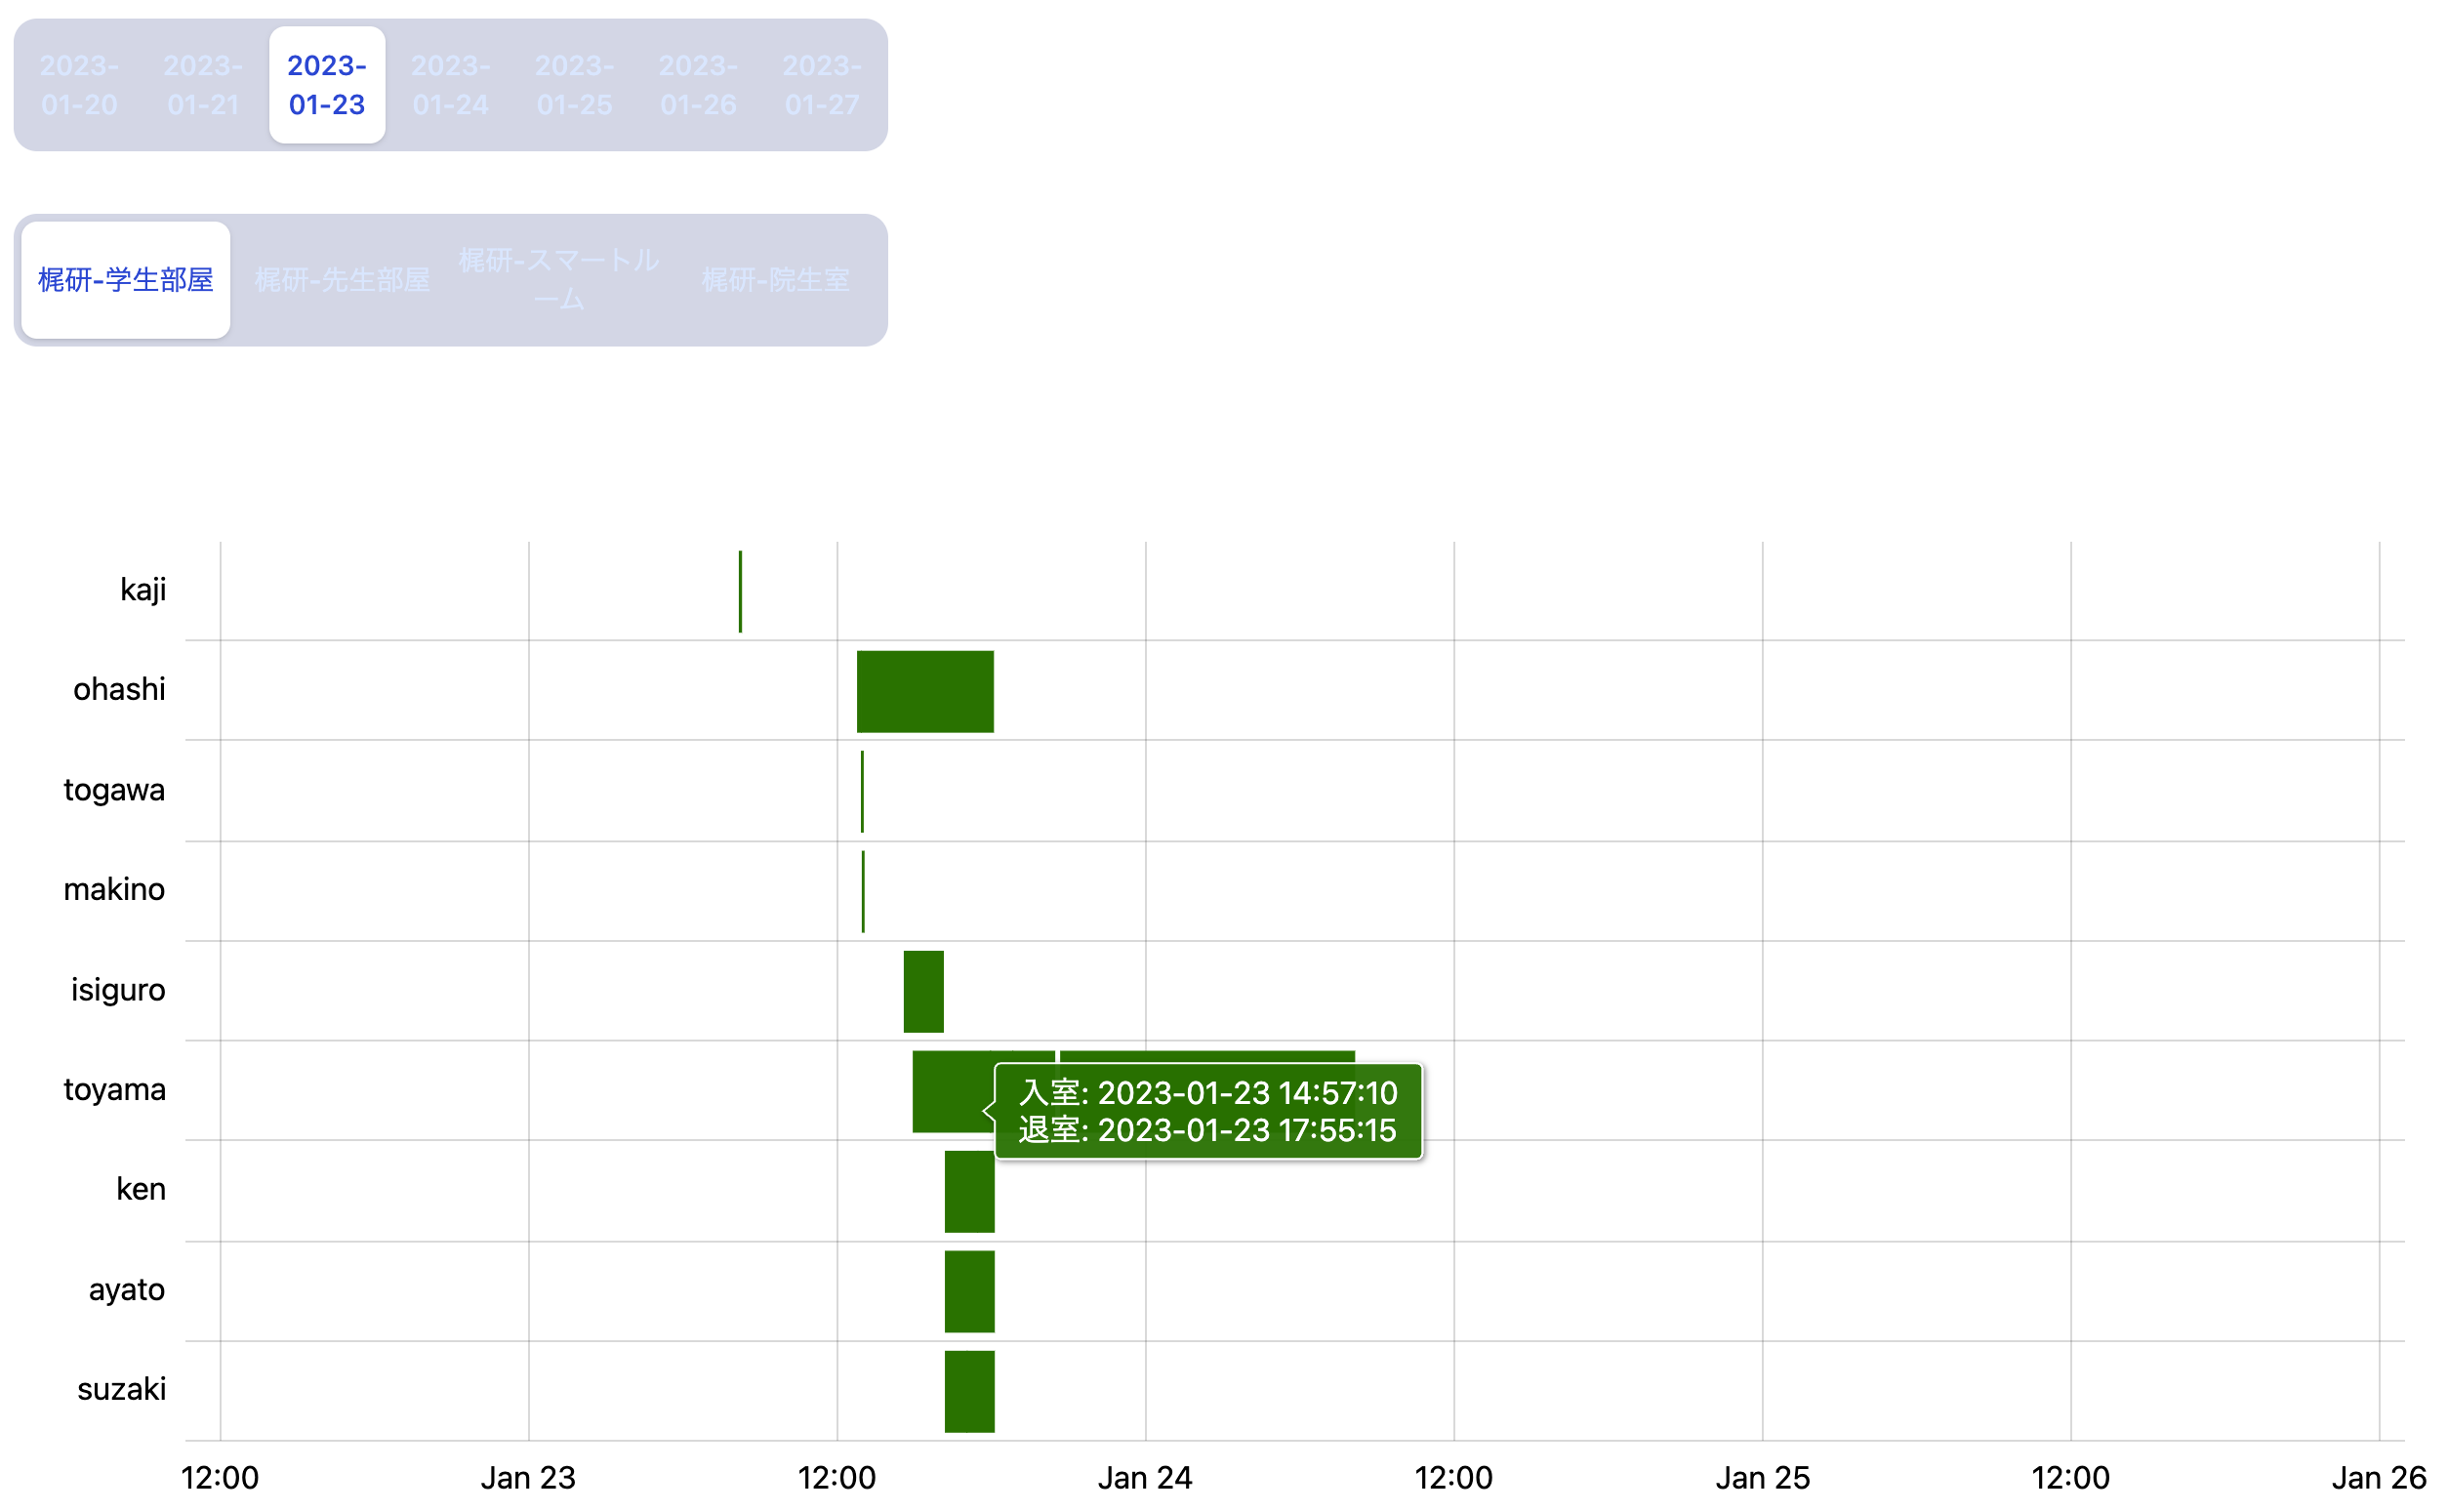
\includegraphics[width=15cm]{image/gantt.png}
  \caption{ガントチャートを用いた在室時間の可視化} \label{fig:gantt}
\end{figure}



また滞在情報をフロアマップ上に可視化を行った.
図\ref{fig:floor}にその画面を示す.
数字が表示されているところにカーソルを合わせると示した図のように,その部屋に在室している利用者の名前が書かれたツールチップが表示される.
既存の滞在ウォッチでは在室者をリスト形式で表示するのみであったが,フロアマップ上に滞在者を可視化によって,在室者の位置を把握しやすくなりコミュニケーション促進につながる可能性が高いと考えられる.


\begin{figure}[tbh]
  \centering
  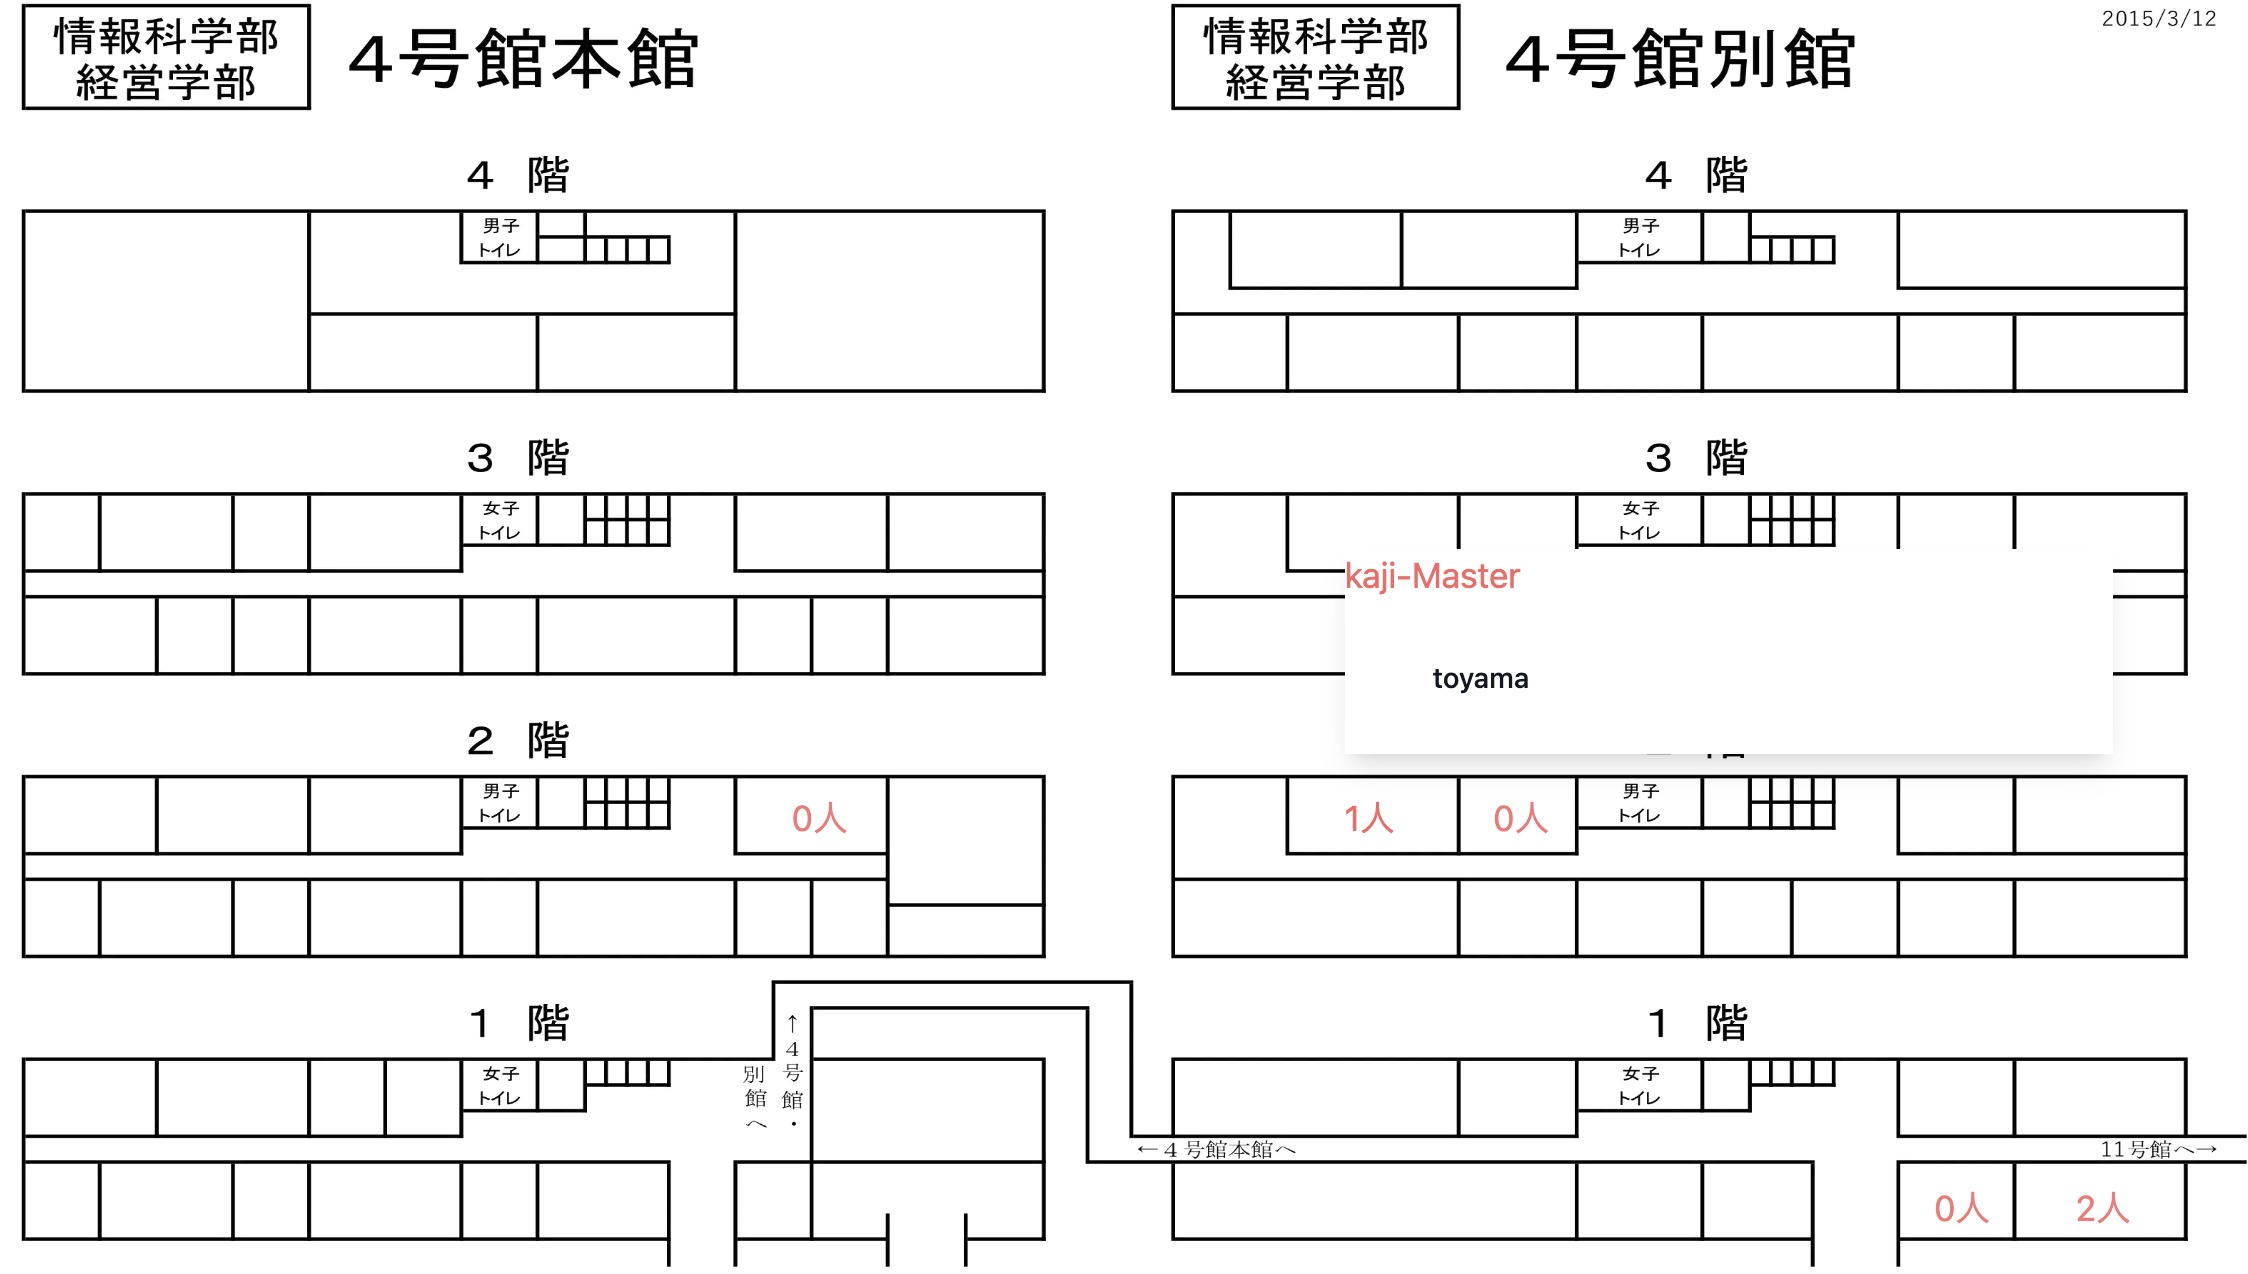
\includegraphics[width=15cm]{image/floorMap.jpg}
  \caption{フロアマップを用いた在室者を可視化} \label{fig:floor}
\end{figure}




















